\section{C. 함수 복원}

\begin{frame} % No title at first slide
    \sectiontitle{C}{함수 복원}
    \sectionmeta{
        \texttt{combinatorics}\\
        출제진 의도 -- \textbf{\color{acplatinum}Medium}
    }
    \begin{itemize}
        \item 제출 406번, 정답 99팀 (정답률 24.63\%)
        \item 처음 푼 팀: \textbf{여기가월파2020인가요} (월파, 치러, 왔어요), 10분
        \item 출제자: \texttt{moonrabbit2}
    \end{itemize}
\end{frame}

\begin{frame}{\textbf{C}. 함수 복원}
    \begin{figure}[h!]
        \centering
        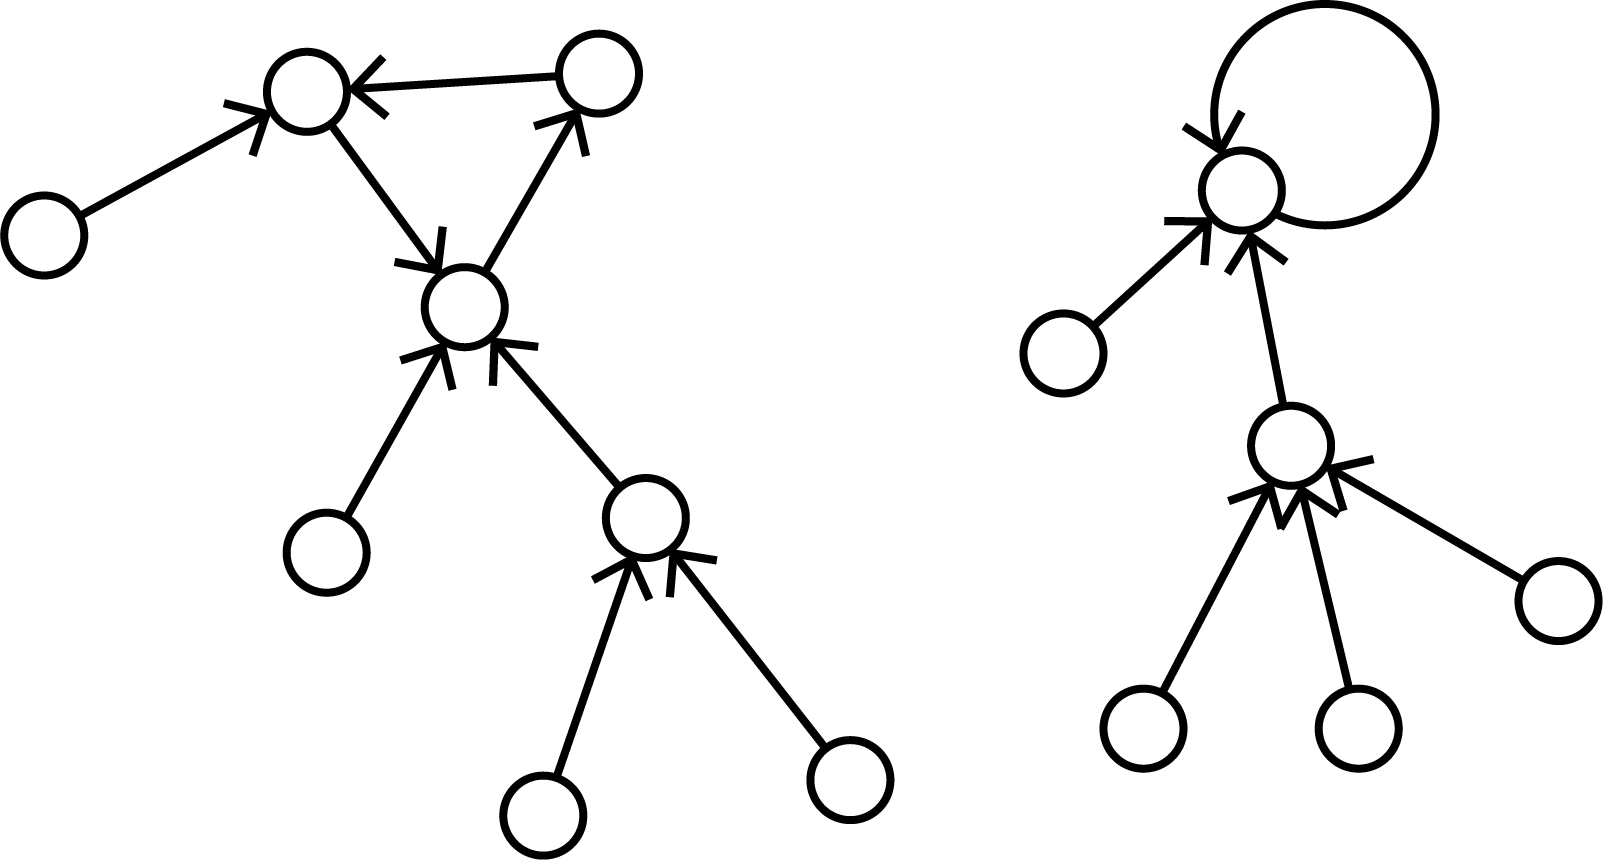
\includegraphics[width=0.5\linewidth]{../images/function-restore/fx-1n.png}
    \end{figure}
    \begin{itemize}
        \item 함수 그래프는 각 컴포넌트가 하나의 사이클에 연결된 트리들로 이루어져 있습니다.
        \item 자기보다 더 적은 수의 정점에 도달할 수 있는 정점이 있다면 트리에 속하고, 그렇지 않으면 사이클에 속하는 정점입니다.
    \end{itemize}
\end{frame}
\begin{frame}{\textbf{C}. 함수 복원}
    \begin{figure}[h!]
        \centering
        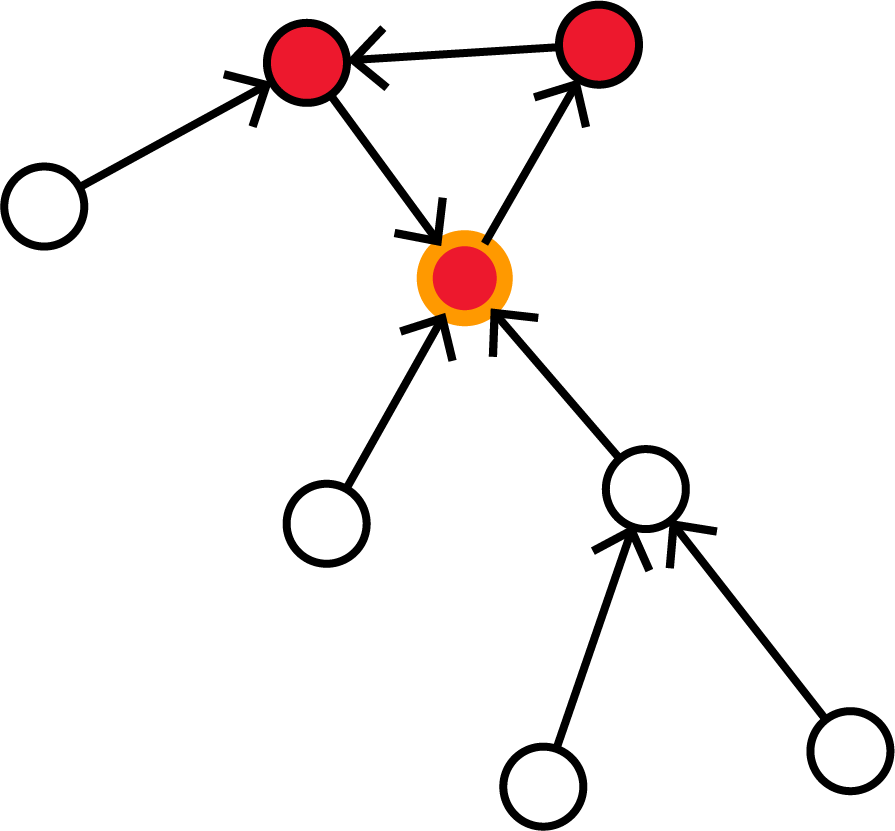
\includegraphics[width=0.35\linewidth]{../images/function-restore/fx-2n.png}
    \end{figure}
    \begin{itemize}
        \item 사이클 정점에서는 사이클 상의 모든 정점이 도달 가능합니다.
        \item 사이클 상의 한 정점을 고정하고, 그 정점으로부터 도달 가능한 정점들을 묶는 것을 반복해 모든 사이클을 구할 수 있습니다,
        \item 각 사이클에 대해, 사이클의 길이가 $L$이라면 원순열 $(L-1)!$을 답에 곱합니다.
    \end{itemize}
\end{frame}
\begin{frame}{\textbf{C}. 함수 복원}
    \begin{figure}[h!]
        \centering
        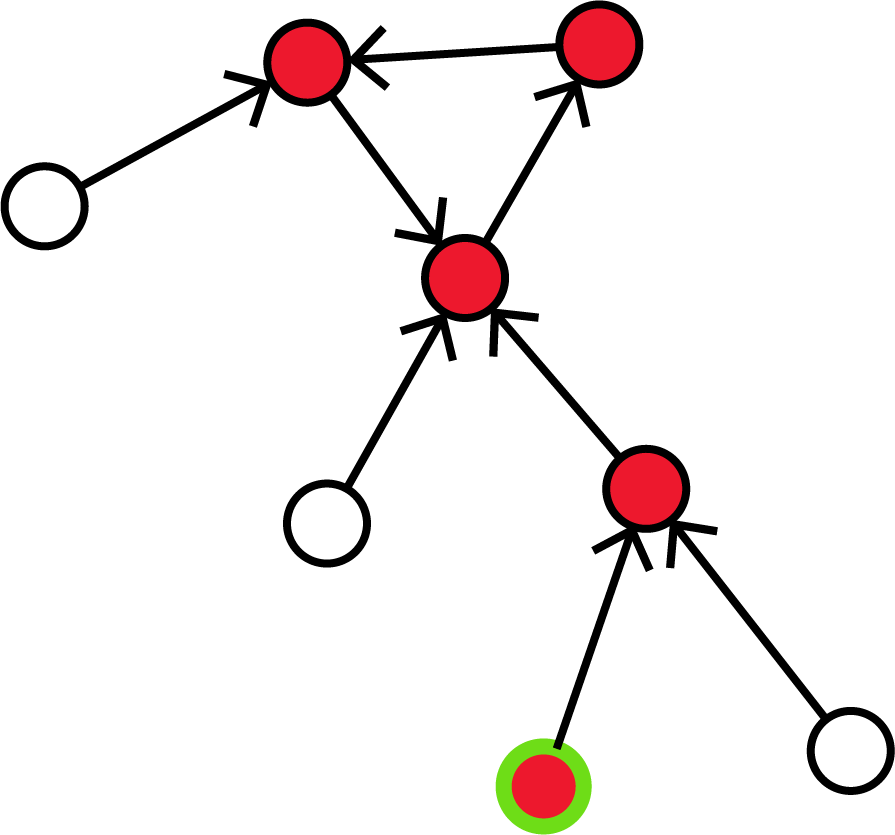
\includegraphics[width=0.35\linewidth]{../images/function-restore/fx-3n.png}
    \end{figure}
    \begin{itemize}
        \item 트리 정점에서는 사이클 상의 정점과 함께 사이클까지의 트리 상의 경로에 있는 정점들이 추가로 도달 가능합니다.
        \item 트리 정점의 부모는 해당 정점보다 도달 가능한 정점의 수가 1 적습니다.
    \end{itemize}
\end{frame}
\begin{frame}{\textbf{C}. 함수 복원}
    \begin{itemize}
        \item 트리 정점에 대해, 부모도 트리 정점이면 부모가 유일하게 고정됩니다.
        \item 부모가 사이클 정점이면 사이클 상의 임의의 정점이 부모가 될 수 있습니다.
        \item 그러므로 부모가 사이클 정점이면 부모가 포함된 사이클의 크기 $L$을 답에 곱합니다.
    \end{itemize}
\end{frame}
\begin{frame}{\textbf{C}. 함수 복원}
    \begin{itemize}
        \item 시간복잡도는 \complexity{N^2}입니다. 제한이 매우 여유롭게 주어져, \complexity{N^3} 풀이도 가능합니다.
        \item 답이 0인지 판별하는 것은 어렵지 않습니다. 온갖 조건문을 넣고 싶지 않다면 실제 함수를 하나 만들면 편하게 구현이 가능합니다. 다만, 이 문제에서는 필요하지 않았습니다.
    \end{itemize}
\end{frame}